\documentclass[12pt,a4paper]{article}
\usepackage{listings}
\usepackage{xcolor}
\definecolor{codegreen}{rgb}{0,0.6,0}
\definecolor{codegray}{rgb}{0.5,0.5,0.5}
\definecolor{codepurple}{rgb}{0.58,0,0.82}
\definecolor{backcolour}{rgb}{0.95,0.95,0.92}
\lstdefinestyle{mystyle}{
    backgroundcolor=\color{backcolour},   
    commentstyle=\color{codegreen},
    keywordstyle=\color{magenta},
    numberstyle=\tiny\color{codegray},
    stringstyle=\color{codepurple},
    basicstyle=\ttfamily\footnotesize,
    breakatwhitespace=false,         
    breaklines=true,                 
    captionpos=b,                    
    keepspaces=true,                 
    numbers=left,                    
    numbersep=5pt,                  
    showspaces=false,                
    showstringspaces=false,
    showtabs=false,                  
    tabsize=2
}
\lstset{style=mystyle}
\usepackage{graphicx}
\graphicspath{ {./Image/2020-03-17/} }
\usepackage{caption} 

\title{Message AlgoTrade}
\author{4T}


\begin{document}
\maketitle
Le but est de créer un modèle IA permettant de se projeter dans le temps. Je lui donne les prix passés, et il doit me prédire les futurs prix à venir EUR/USD. Utilisation entre autre de Keras == 2.1.5 basé sur Tensorflow == 1.5.0.

\section*{Organisation}
2 Objets :
\begin{itemize}
	\item Ia Object, contenant le modèle de l'IA
	\item Price Object, contenant les prix de mai 2000 à septembre 2019
\end{itemize}


Un programme main centralise toutes les données afin d’entraîner le modèle.
 
\newpage
\section*{17/03/2020}

\subsection*{Configurations}
Le modèle est composé de multiples layers avec des activations sigmoids et linéaires (indispensable pour garder la valeur du prix par delà les layers) : \\
\begin{lstlisting}[language=Python, caption=Modèle d'organisation layers]
val_input = Input(shape=(120,), name="input")
x = Dense(256, activation="linear")(val_input)
x = Dense(512, activation="sigmoid")(x)
x = Dense(512, activation="softplus")(x)
x = Dense(1024, activation="linear")(x)
x = Dense(1024, activation="softplus")(x)
x = Dense(512, activation="sigmoid")(x)
x = Dense(256, activation="linear")(x)
val_output = Dense(30, activation="linear", name="output")(x)
\end{lstlisting}

Les configurations pour l'optimizer SGD (Stochastic Gradient Descent) : \\
\begin{tabular}{ l c r }
   	Loss & 'MSE' Mean Suare Error & (Best) \\
	Learning Rate & 0.01 & (à réduire) \\
	Decay & 10e-6 & (tester autre) \\
	Momentum & 0.9 & (comprendre) \\
	Nesterov & True & (lié à momentum) \\
\end{tabular}

\subsection*{Résultats}
Après 14 entraînements sur 10 000 datas (renouvelés à chaque entraînement), de cycle de 100 epochs, on observe que les prédictions se rapprochent des prix réels, même si le modèle ne s'est jamais entraîné sur les datas données. Cependant, les prédictions du modèles après le 14 ème entraînement ne sont pas aussi bonnes que celles du 9ème (meilleur modèle sur les tests effectués).

\begin{center}
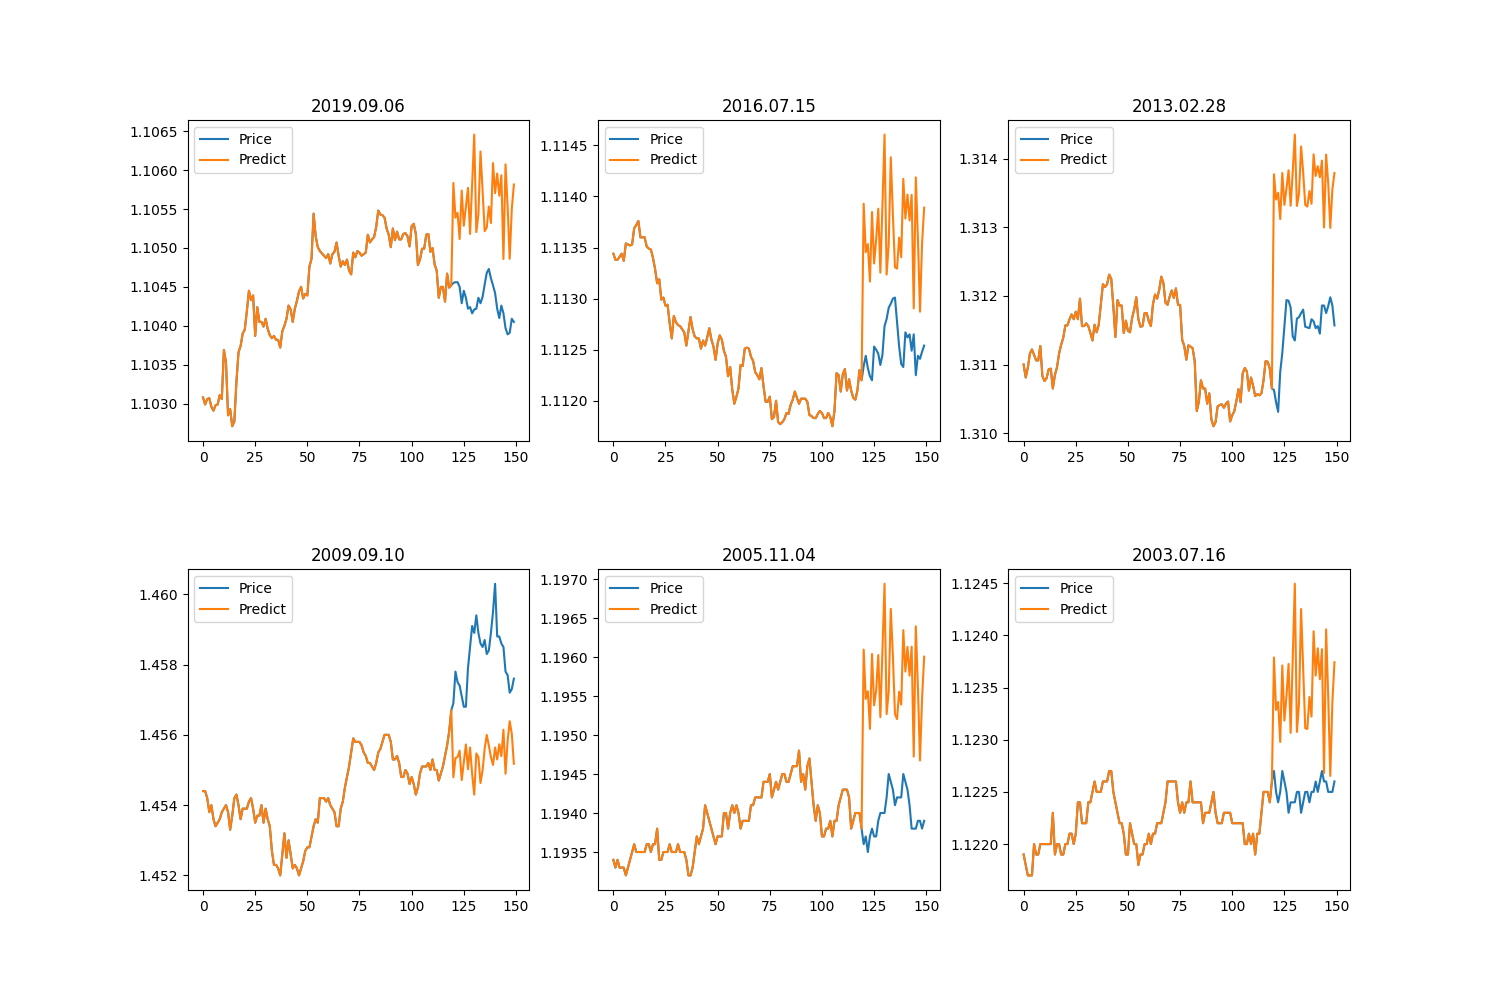
\includegraphics[scale=0.25,trim={0 2cm 0 0},clip]{1-2020-03-18.png} 
\\1ère Entrainement : Prédictions très éloignées de la réalité
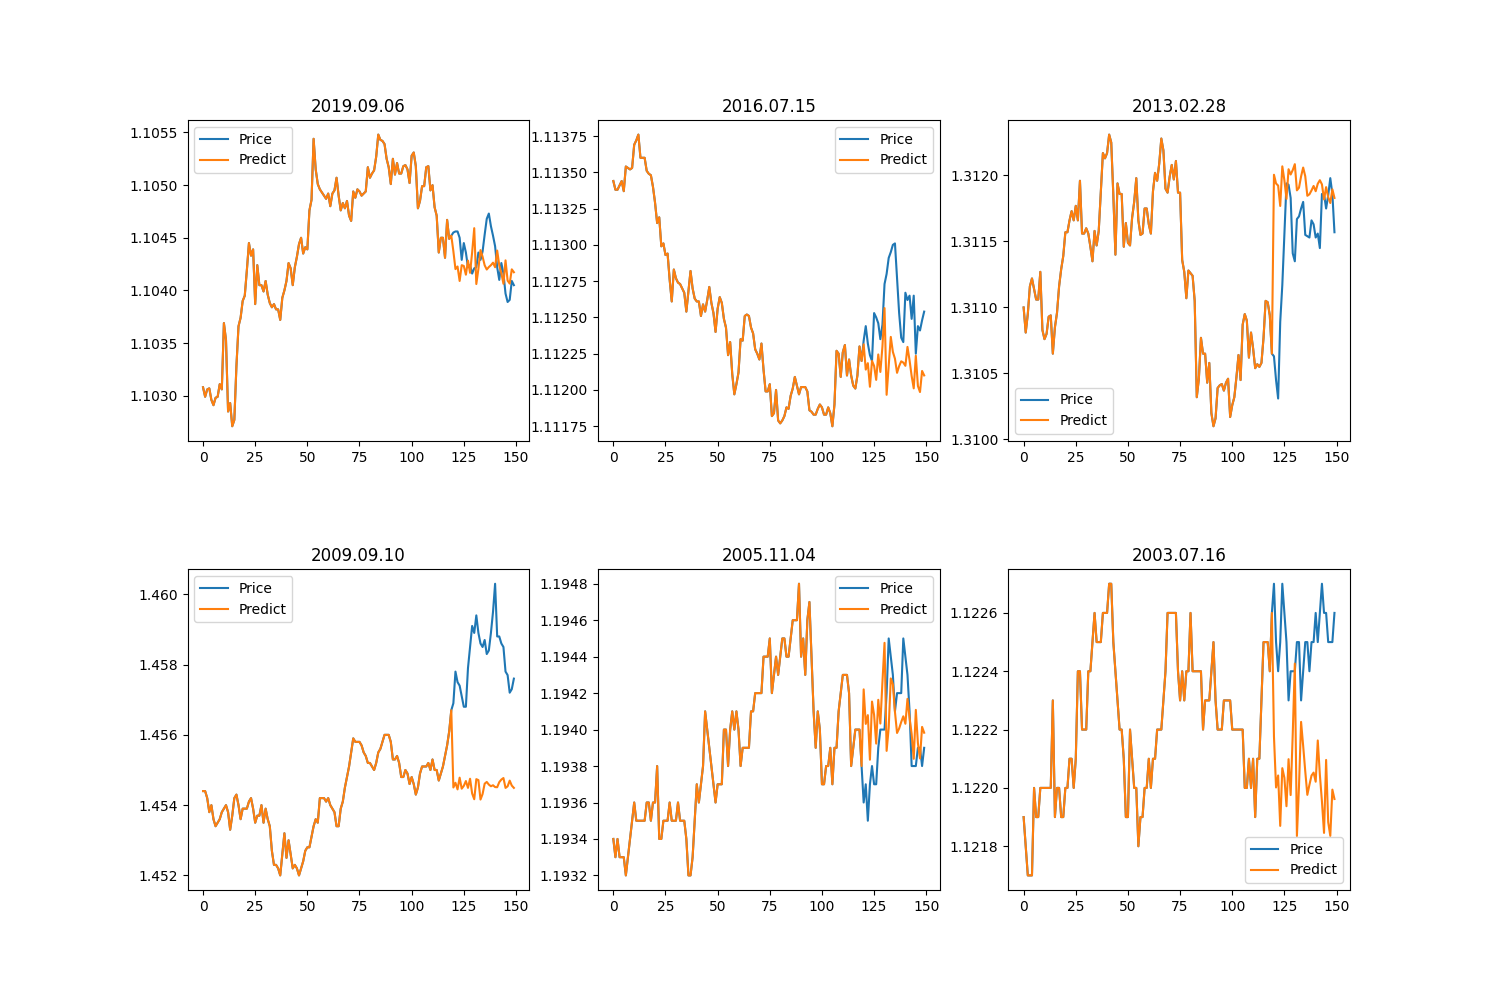
\includegraphics[scale=0.25,trim={0 2cm 0 0},clip]{9-2020-03-18.png} 
\\9ème Entrainement : Prédictions plutôt proche de la réalité, sauf en 2009 et 2003. Mais les prédictions en 2013 et 2019 sont très encourageantes !!!
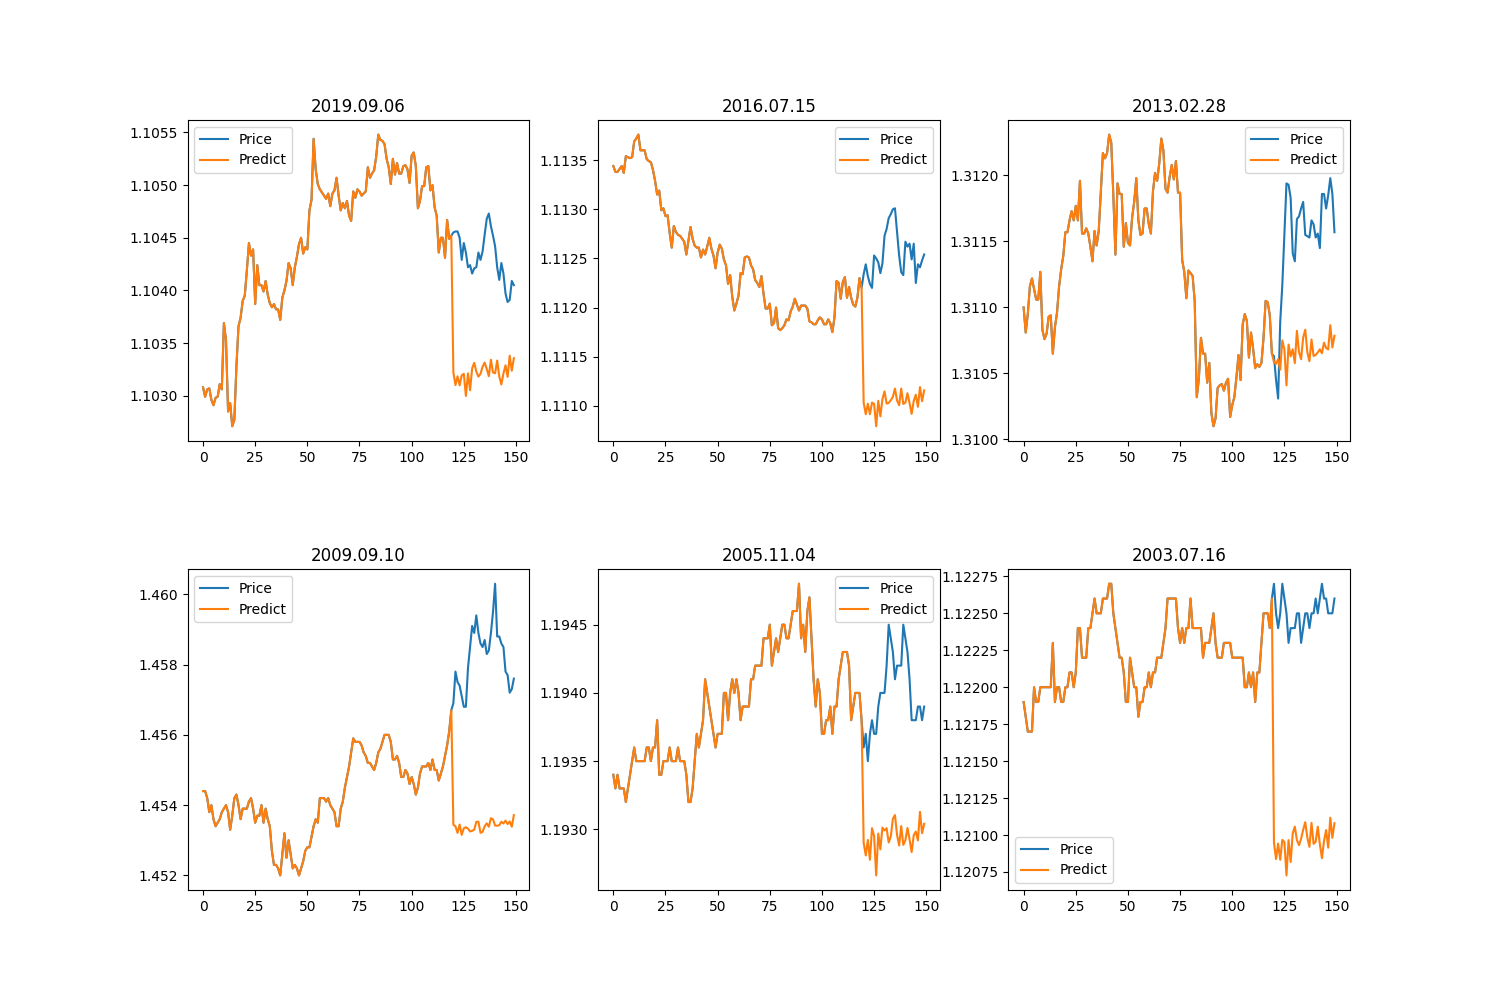
\includegraphics[scale=0.25,trim={0 2cm 0 0},clip]{14-2020-03-18.png} 
\\14ème Entrainement : Prédictions sont totalement fausses, on a entraîné le modèle trop longtemps, "OverFitting"
\end{center}

Afin de réduire cet Overfitting, nous allons essayer de réduire plus rapidement le Learning Rate, et essayer de comprendre l'utilisation du Momentum. Afin de gagner du temps nous allons reprendre les entraînements à partir du modèle numéro 9 (6h45min d'entraînement), et poursuivre l'entraînement avec des modifications à venir.

 
\newpage
\section*{19/03/2020}
\subsection*{Gros Entraînement}
Au vu des dernières analyses, le modèle a été lancé pour un entraînement intensif sur 1.000.000 données pour 100 epochs. Le learning rate a été réduit, et j'espère que l'entraîner simultanément sur autant de donnée permettra au modèle d'acquérir des résultats plus convaincants. Le temps total d'apprentissage est estimé à 3 jours, étant lancé le 18, j'espère finir l'entraînement d'ici demain. Afin de mettre en pratique mon idée de structuration de modèle.

\subsection*{Structuration}
L'idée est d'allé encore plus loin dans l'utilisation du Deep learning. Jusqu'ici, le seul objectif était de prédire les données futures. Mais ensuite, il va falloir prendre des décision d'achat, de vente, ou ne rien faire sur ces données. Donc Autant créer une IA pour faire cela également. Ainsi les prix prédit par la première Intelligence Artificielle entrerait en Input dans les Modèles suivant :
\begin{itemize}
	\item Ordre d'action (Achat, Vente, Attendre) soit sous forme de classification, soit en pondérant les meilleurs prédictions par des float
	\item Conseil de Take Profit et Stop Loss, et pous l'achat, et pour la vente.
\end{itemize}


\begin{huge}
\begin{center}
Suite à venir !!!

\end{center}
\end{huge}


\end{document}